\documentclass[reqno]{amsart}
\setlength{\parindent}{0pt}
\usepackage{graphicx}
\title{Simulated TGA curves}
\begin{document}
\maketitle

The Arrhenius pyrolysis model from Morvan and Dupuy 2001 (Combustion and Flame) written for TGA curves is

\begin{align}
\frac{d}{dT} \alpha_s \rho_s Y_{H2O} &=\frac{1}{dT/dt}\frac{k_{H2O}}{\sqrt{T_s}} \alpha_s\rho_s Y_{H2O} \exp(-E_{H2O}/(RT_s)) \,,\\
\frac{d}{dT} \alpha_s \rho_s Y_{i} &=\frac{1}{dT/dt}k_{pyr}\alpha_s\rho_s Y_i \exp(-E_{pyr}/(RT_s)) \,,\\
\frac{d}{dT} M_{O_2} &=\frac{1}{dT/dt}k_{char} M_{O_2} \exp(-E_{char}/(RT_s))\alpha_s \sigma_s \,,\\
%          -(1/dTdt)*kchar*y(3)*exp(-erchar./t)*y(4)*sigs./y(5);...
\frac{d}{dT} \alpha_s &=\frac{1}{dT/dt}\frac{k_{char}}{\rho_s}\alpha_s \exp(-E_{char}/(RT_s)) \,,\\
\frac{d}{dT} \rho_s &=\frac{1}{dT/dt}\big((\nu_{char}-\nu_{soot}-1  k_{pyr} \alpha_s \rho_s Y_i \exp(-E_{pyr}/(RT_s)) \nonumber \\
                    & -\frac{k_{H2O}}{\sqrt{T_s}} \alpha_s\rho_s Y_{H2O} \exp(-E_{H2O}/(RT_s))\big) \,,\\
\frac{d}{dT} \alpha_s \rho_s Y_{char} &=\frac{1}{dT/dt}\big( (\nu_{char}-\nu_{soot}) k_{pyr}\alpha_s\rho_s Y_i \exp(-E_{pyr}/(RT_s)) \nonumber \\
&-(\nu_{ash}/\nu_{char}+1) k_{char} M_{O_2} \exp(-E_{char}/(RT_s))\alpha_s \sigma_s \,.
\label{eqn:TGAmodel}
\end{align}

Notice that quantities like $\alpha\rho Y$ are masses of particular species. 
Once we have solved the system of equations, we can compute the individual mass fractions and we can reconstruct the mass loss curve by looking at mass as a function of solid temperature $T_s$. 
In TGA the heating rate is constant and the atmosphere is initially inert.

In MD01 there is a typing error: $\dot{\omega}^2_{H2O}$ instead of $\dot{\omega}^s_{H2O}$.

The parameters are shown in table \ref{tab:parameters}.
This simulation is for pine needles at a realistic $10\,K/min$ (again a typo in MD01) heating rate. 
The model was implimented in Matlab using the ode45 solver because it was highest order stable solver. 
ode23 was also stable. 
ode45 is a variable, $4^{th}-$ or $5^{th}-$ order Runge-Kutta scheme.
The simulated curves are shown in figure \ref{fig:simulatedTGA}, this should be compared with figure $3$ in MD01.

\newpage

%all the constants
\begin{table}
\centering
\begin{tabular}{c c l}
\hline
  $\sigma_s$ & $4000$ & Surface to volume ratio \\
  $dT/dt$ & $10/60$ & Heating rate $K/min$\\
\hline
  Pre-exponential factors & &\\ 
  $k_{H2O}$ & $6.05\times 10^5$ & $K^{1/2}s^{-1}$\\
  $k_{pyr}$ & $3.64\times 10^3$ & $s^{-1}$ \\
  $k_{char}$& $430$ & $ms^{-1}$ \\
%
\hline
  Stoichiometric ratios & &\\
  $\nu_{char}$ & $0.338$& \\ %char
  $\nu_{CO_2}$ & $0.2$&\\ %carbon dioxide
  $\nu_{ash}$ & $0.033$&\\ %ash
  $\nu_{soot}$ & $0.05$&\\ %soot
  $\nu_{O_2}$ & $8/3$&\\ %oxygen
%
\hline
 Activation energies & & \\
  $E_{H2O}/R$ & $5956$ & $K$ \\
  $E_{pyr}/R$ & $7250$ & $K$ \\
  $E_{char}/R$& $9000$ & $K$ \\
%
\hline
   Initial conditions & & \\
   $\rho(0)$ & $800$ & Material density $kg/m^3$\\
   $\alpha(0)$ & $0.5$ & Occupied volume $1/m$\\
   $M_{O_2}(0)$ & $0$ & Mass of oxygen $kg$ \\
   $Y_{H2O}(0)$ & $0.1$ & Moisture content\\
   $Y_{i}(0)$ & $0.9$ & Dry wood\\
   $Y_{char}$ & $0$ & Char \\
\hline
\end{tabular}
\caption{Parameters used in the simulated TGA experiments}
\label{tab:parameters}
\end{table}

\begin{figure}
\centering
  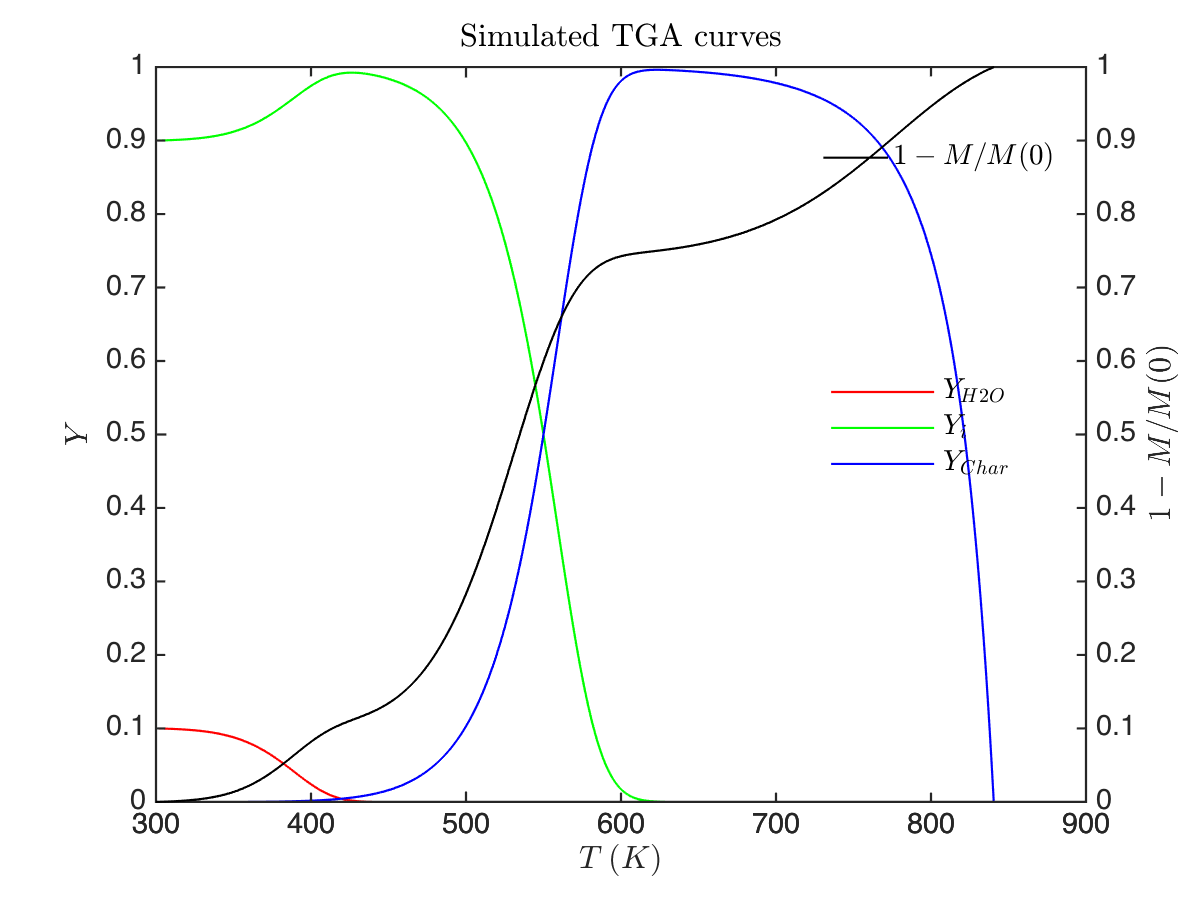
\includegraphics[scale=0.5]{simulatedTGA.png}
\caption{Reproduction of MD01 figure 3 TGA data}
\label{fig:simulatedTGA}
\end{figure}
\end{document}
